%----------------------------------------------------------------
%
%  File    :  thesis.tex
%
%  Authors :  Keith Andrews, IICM, TU Graz, Austria
%             Manuel Koschuch, FH Campus Wien, Austria
%			  Sebastian Ukleja, FH Campus Wien, Austria
% 
%  Created :  22 Feb 96
% 
%  Changed :  14 Oct 2020
%
%  For suggestions and remarks write to: sebastian.ukleja@fh-campuswien.ac.at 
%----------------------------------------------------------------

% --- Setup for the document ------------------------------------

%Class for a book like style:
\documentclass[11pt,a4paper,oneside]{scrbook}
%For a more paper like style use this class instead:
%\documentclass[11pt,a4paper,oneside]{thesis}

%input encoding for windows in utf-8 needed for Ä,Ö,Ü etc..:
\usepackage[utf8]{inputenc}
%input encoding for linux:
%\usepackage[latin1]{inputenc}
%input encoding for mac:
%\usepackage[applemac]{inputenc}

\usepackage[ngerman]{babel}
%for english use this instead:
%\usepackage[english]{babel}

\usepackage{csquotes}
\MakeOuterQuote{"}

\usepackage{float}

\usepackage{minted}

%needed for font encoding
\usepackage[T1]{fontenc}

% want Arial? uncomment next two lines...
%\usepackage{uarial}
%\renewcommand{\familydefault}{\sfdefault}

%some formatting packages
\usepackage[bf,sf]{subfigure}
\renewcommand{\subfigtopskip}{0mm}
\renewcommand{\subfigcapmargin}{0mm}

%For better font resolution in pdf files
\usepackage{lmodern}

\usepackage{url}

%\usepackage{latexsym}

\usepackage{geometry} % define pagesize in more detail

% --- Settings for header and footer ---------------------------------
\usepackage{scrlayer-scrpage}
\clearscrheadfoot
\pagestyle{scrheadings}
\automark{chapter}

%Left header shows chapter and chapter name, will not display on first chapter page use \ihead*{\leftmark} to show on every page
\ihead{\leftmark} 	
%\ohead*{\rightmark}	%optional right header
\ifoot*{Markus Mayer}	%left footer shows student name
\ofoot*{\thepage}		%right footer shows pagination
%---------------------------------------------------------------------

\usepackage{colortbl} % define colored backgrounds for tables

\usepackage{courier} %for listings
\usepackage{listings} % nicer code formatting
\lstset{basicstyle=\ttfamily,breaklines=true,breakatwhitespace}
\let\oldlstinline\lstinline
\renewcommand{\lstinline}[1]{\sloppy\oldlstinline{#1}}

\usepackage[dvipsnames]{xcolor}

\definecolor{groovyblue}{HTML}{0000A0}
\definecolor{groovygreen}{HTML}{008000}
\definecolor{darkgray}{rgb}{.4,.4,.4}
 
\lstdefinelanguage{Groovy}[]{Java}{
  keywordstyle=\color{groovyblue}\bfseries,
  stringstyle=\color{groovygreen}\ttfamily,
  keywords=[3]{each, findAll, groupBy, collect, inject, eachWithIndex},
  morekeywords={def, as, in, use},
  moredelim=[is][\textcolor{darkgray}]{\%\%}{\%\%},
  moredelim=[il][\textcolor{darkgray}]{§§}
}

\lstdefinelanguage{Kotlin}{
  comment=[l]{//},
  commentstyle={\color{gray}\ttfamily},
  emph={filter, first, firstOrNull, forEach, lazy, map, mapNotNull, println},
  emphstyle={\color{OrangeRed}},
  identifierstyle=\color{black},
  keywords={!in, !is, abstract, actual, annotation, as, as?, break, by, catch, class, companion, const, constructor, continue, crossinline, data, delegate, do, dynamic, else, enum, expect, external, false, field, file, final, finally, for, fun, get, if, import, in, infix, init, inline, inner, interface, internal, is, lateinit, noinline, null, object, open, operator, out, override, package, param, private, property, protected, public, receiveris, reified, return, return@, sealed, set, setparam, super, suspend, tailrec, this, throw, true, try, typealias, typeof, val, var, vararg, when, where, while},
  keywordstyle={\color{NavyBlue}\bfseries},
  morecomment=[s]{/*}{*/},
  morestring=[b]",
  morestring=[s]{"""*}{*"""},
  ndkeywords={@Deprecated, @JvmField, @JvmName, @JvmOverloads, @JvmStatic, @JvmSynthetic, Array, Byte, Double, Float, Int, Integer, Iterable, Long, Runnable, Short, String, Any, Unit, Nothing},
  ndkeywordstyle={\color{BurntOrange}\bfseries},
  sensitive=true,
  stringstyle={\color{ForestGreen}\ttfamily},
}

\usepackage{graphicx}
  \pdfcompresslevel=9
  \pdfpageheight=297mm
  \pdfpagewidth=210mm
  \usepackage[         % hyperref should be last package loaded
    pdftex, 		   % needed for pdf compiling, DO NOT compile with LaTeX
    bookmarks,
    bookmarksnumbered,
    linktocpage,
    pagebackref,
    pdfview={Fit},
    pdfstartview={Fit},
    pdfpagemode=UseOutlines,                 % open bookmarks in Acrobat
  ]{hyperref}
\DeclareGraphicsExtensions{.pdf,.jpg,.png}
\usepackage{bookmark}

\usepackage[title]{appendix}

%paper format
\geometry{a4paper,left=30mm,right=25mm, top=30mm, bottom=30mm}

\setlength{\parskip}{3pt plus 1pt minus 0pt}       % vert. space before a paragraph

\setcounter{tocdepth}{1}        % lowest section level entered in ToC
\setcounter{secnumdepth}{2}     % lowest section level still numbered

%Start of your document beginning with title page
\begin{document}

% --- Main Title Page ------------------------------------------------
\begin{titlepage}
\frontmatter
\begin{picture}(50,50)
\put(-70,40){\hbox{
\includegraphics{images/logo.png}}}
\end{picture}

\vspace*{-5.8cm}

\begin{center}

\vspace{6.2cm}

\hspace*{-1.0cm} {\LARGE \textbf{Titel \\}}
\vspace{0.2cm}
\hspace*{-1.0cm} Untertitel \\

\vspace{2.0cm}

\hspace*{-1.0cm} { \textbf{Bachelorarbeit\\}}

\vspace{0.65cm}

\hspace*{-1.0cm} Eingereicht in teilweiser Erfüllung der Anforderungen zur Erlangung des akademischen Grades: \\

\vspace{0.65cm}

\hspace*{-1.0cm} \textbf{Bachelor of Science in Engineering\\}

\vspace{0.65cm}

\hspace*{-1.0cm} an der FH Campus Wien \\
\vspace{0.2cm}
\hspace*{-1.0cm} Studienfach: Computer Science and Digital Communications \\

\vspace{1.6cm}

\hspace*{-1.0cm} \textbf{Autor:} \\
\vspace{0.2cm}
\hspace*{-1.0cm} Markus Mayer \\

\vspace{0.7cm}

\hspace*{-1.0cm} \textbf{Matrikelnummer:}\\
\vspace{0.2cm}
\hspace*{-1.0cm} 52006537 \\

\vspace{0.7cm}

\hspace*{-1.0cm} \textbf{Betreuer:} \\
\vspace{0.2cm}
\hspace*{-1.0cm} MSc René Goldschmid \\

\vspace{0.7cm}

% Reviewer if needed:
%\hspace*{-1.0cm} \textbf{Reviewer: (optional)} \\
%\vspace{0.2cm}
%\hspace*{-1.0cm} Titel Vorname Nachname \\


\vspace{1.0cm}

\hspace*{-1.0cm} \textbf{Datum:} \\
\vspace{0.2cm}
\hspace*{-1.0cm} 25.09.2022 \\

\end{center}
\end{titlepage}

\newpage

\setcounter{page}{1}

\vspace*{16cm}

% --- Declaration of authorship --------------------------------------------
\hspace*{-0.7cm} \underline{Erklärung der Urheberschaft:}\\\\
Ich erkläre hiermit diese Bachelorarbeit eigenständig verfasst zu haben. Ich habe keine anderen Quellen, als die in der Arbeit gelisteten verwendet, noch habe ich jegliche unerlaubte Hilfe in Anspruch genommen\\\\
Ich versichere diese Bachelorarbeit in keinerlei Form jemandem Anderen oder einer anderen Institution zur Verfügung gestellt zu haben, weder in Österreich noch im Ausland.\\\\
Weiters versichere ich, dass jegliche Kopie (gedruckt oder digital) identisch ist.
\\\\\\
Datum: \hspace{6cm} Unterschrift:\\

% --- English Abstract ----------------------------------------------------
\cleardoublepage
\chapter*{Abstract}
(E.g. ``This thesis investigates...'')


% --- German Abstract ----------------------------------------------------

\cleardoublepage
\chapter*{Kurzfassung}
(Z.B. ``Diese Arbeit untersucht...'')

% --- Abbrevations ----------------------------------------------------
\newpage\noindent
\chapter*{Abkürzungen}
\vspace{0.65cm}

\begin{table*}[htbp]
		\begin{tabular}{ll}
			OHA      & Open Handset Alliance \\
			OAA      & Open Automotive Alliance \\
            LiPS     & Linux Phone Standards Forum  \\
            OMA      & Open Mobile Alliance \\
            IDE      & Integrated Development Enviroment \\
            DSL      & Domain Specific Language \\
            DAO      & Data Access Object \\
		\end{tabular}
\end{table*}

% --- Key terms ----------------------------------------------------
\newpage
\chapter*{Schlüsselbegriffe}
\vspace{0.65cm}

\begin{itemize}
	\setlength{\itemsep}{0pt}
	\item[] 1
	\item[] 2
	\item[] 3
\end{itemize}

% --- Table of contents autogenerated ------------------------------------
\newpage
\tableofcontents

% --- Begin of Thesis ----------------------------------------------------
\mainmatter
\chapter{Einführung}
\section{Motivation}
Warum ist diese Arbeit interessant?
\section{Relevanz}
Inwiefern ist diese Arbeit neu und wichtig?


\chapter{Hauptteil}

\section{Android-Übersicht}

Um einen Überblick über Android zu bekommen, beziehungsweise wo der Fokus eines der am weitest verbreitetsten Betriebssysteme für mobile Geräte liegt, muss man etwas in die Vergangenheit blicken. Android ist ein Open-Source-Betriebssystem, welches auf einem Linux-Kernel basiert. Es wurde von der Firma Android Inc. entwickelt, die im Jahr 2005 von Google übernommen wurde \cite{hrmoandroid}.


\subsection{Rückblick}

Im Jahr 2006 hatten Hersteller, die ein Smartphone auf den Markt bringen wollten, die Möglichkeit teure Lizenzgebühr für ein Betriebssystem zu bezahlen oder ein eigenes Betriebssystem zu entwickeln. Google gründet 2007 die Open Handset Alliance (OHA) und führt Android als Open Source-Plattform ein. Im Jahr 2008 wird Android auf die Version mit dem Namen Cupcake aktualisiert. Bei dieser Version können Hersteller wie HTC und Samsung, aber auch Mobilfunkanbieter das Betriebssystem ihrer Smartphones anpassen. Laut Google kommt 2010 Android auf 34 Mobilgerätetypen in 49 Ländern zum Einsatz und bietet damit den Nutzern eine größere Auswahl als je zuvor. 2011 veröffentlicht Google mit Android 3.0 Honeycomb ein für Tablets optimiertes Betriebssystem, das als Basis für das Betriebssystem Fire OS des Kindle Fire-Tablets von Amazon dient. Der sogenannte Android Market wird 2012 in Google Play umbenannt und Entwickler*innen können weiterhin ihre Apps in wenigen Stunden veröffentlichen. Zusätzlich zur Unterstützung von Mobilgeräten wird 2014 die Open Automotive Alliance (OAA) gegründet, deren Ziel es ist Android auch für Autos zu nutzen. Heute sind 45 führende Automarken Mitglied der OAA. Durch die Innovationskraft einiger Hersteller sind 2015 inzwischen Android Geräte für weniger als 50 US-Dollar verfügbar. Mit Stand 2016 gibt es fast 24.000 Android Geräte von über 1.300 Marken. Außerdem gibt es heute dutzende weltweit operierende Stores für Android-Apps. \cite{android.com}


\subsection{Ziele}

Androids Ziele sind zwar ähnlich zu denen des Linux Phone Standards Forum (LiPS) oder der Open Mobile Alliance (OMA), da aber der Ansatz des kompletten Software-Stacks von Android weit über den Fokus dieser standarddefinierenden Organisationen hinausgeht, ist Android kein Teil dieser Organisationen. Verglichen mit dem iPhone, dass eine vollständig herstellerspezifische Hardware- und Softwareplattform ist, die von einem einzigen Unternehmen herausgegeben wird, ist Android ein Open Source-Software-Stack, der von der OHA entwickelt und unterstützt wird und auf jedem kompatiblen Gerät funktionieren soll. \cite{meier_hello_android}


\subsection{Unterstützte Programmiersprachen}

Bis 2019 war Java die offizielle Standardprogrammiersprache für die Entwicklung von Android Apps. Als 2017 Kotlin als unterstützte Sprache für die Android Entwicklung angekündigt wurde, gab es zu Beginn große Aufregung unter den Entwicklern*innen. Jedoch ist die Anzahl der Entwickler*innen die Kotlin verwenden in kürzester Zeit so gestiegen, dass im Jahr 2019 Kotlin, Java als offizielle Standardprogrammiersprache ablöste. \cite{ android_kotlin}

Mit Javas Ablöse als Standardprogrammiersprache wurde seitens Android jedoch weiterhin der offizielle Support für Java und C++ zugesichert \cite{ android_languages}. Das Feedback, dass direkt von den Entwicklern*innen kommt hebt folgende Vorteile bei der Verwendung von Kotlin hervor, wie unter "Android’s Kotlin-first approach" beschrieben \cite{developer.android.com/kotlin/first}.

\begin{itemize} 
  \item \textbf{Ausdrucksstark und prägnant} \\ 
        Es kann mit weniger Code mehr erreicht werden. Codesegmente, die ohne Änderung immer wieder verwendet werden, fachsprachlich auch Boilerplate-Code genannt, können merkbar reduziert werden. Somit kann Kotlin die Produktivität der Entwickler*innen erhöhen. 
  \item \textbf{Sicherer Code} \\ 
        Kotlin enthält viele Sprachfunktionen, die dabei helfen häufige Programmierfehler, wie zum Beispiel Null Pointer Exceptions zu vermeiden. Android Apps mit Kotlin Code haben eine 20-prozentige geringere Absturzwahrscheinlichkeit. 
  \item \textbf{Interoperabel} \\ 
        Kotlin ist zu 100 Prozent interoperabel mit der Programmiersprache Java, dass heißt das Java Code in Kotlin verwendet werden kann und Kotlin Code auch problemlos von Java aus verwendet werden kann. Damit können die Entwickler*innen so viel oder so wenig Kotlin Code in ihren Projekten verwenden, wie sie möchten. 
  \item \textbf{Strukturierte Gleichzeitigkeit} \\ 
        Mit Kotlin Coroutines ist das Arbeiten mit asynchronem Code genauso einfach wie mit blockierendem Code. Diese Coroutines vereinfachen die Verwaltung von diversen Hintergrundaufgaben.
\end{itemize}


\subsection{Android Studio}

Android Studio ist seit 2013 die offizielle Integrated Development Environment (IDE) von Google für die Android-Softwareentwicklung. Um Android Studio zu entwickeln, ging Google eine Kooperation mit der tschechischen Firma JetBrains ein, die zu diesem Zeitpunkt mit IntelliJ IDEA eine der fortschrittlichsten Java IDEs am Markt hatten und auch heute noch haben. Android Studio basiert auf dieser leistungsstarken Entwicklungsumgebung, die von Google mit speziellen Funktionen für die Android-Entwicklung erweitert und angepasst wurde. Eine dieser Funktionen ist ein Build-System, das auf Gradle basiert und mit dem Android Gradle Plugin um einige Features erweitert wurde. Die aktuelle Version zum Zeitpunkt der Arbeit ist Android Studio Dolphin mit dem Versionscode 2021.3.1. Android Studio ist ein Open Source Projekt und steht auch frei zum Download zur Verfügung. \cite{android_studio}


\subsection{Gradle}

Gradle ist ein Build-Management-Automatisierungstool, das den automatischen Download und die Konfiguration von Abhängigkeiten und anderen Bibliotheken übernimmt \cite{Hassan2018}. Gradle stellt im Allgemeinen Standardwerte für Einstellungen und Eigenschaften bereit, daher ist der Einstieg für Entwickler*innen einfacher als bei Systemen wie Ant oder Maven, die davor die Standard Build-Systeme bei Android-Projekten waren. Wenn ein neues Projekt mit Android Studio angelegt wird, werden standardmäßig drei Gradle Files generiert. \cite{Pelgrims2015_1} Die Dateien settings.gradle und build.gradle befinden sich im Stammverzeichnis und eine weitere build.gradle Datei wird im App Ordner angelegt. Die build.gradle Datei im Stammverzeichnis wirkt sich auf jedes Modul des Projekts aus und die build.gradle Datei im App Ordner wirkt sich nur auf das App Modul aus.  In der settings.gradle Datei werden die Repository-Einstellungen auf Projektebene definiert und Gradle mitgeteilt, welche Module bei Erstellung der Anwendung inkludiert werden sollen. Diese Gradle Dateien werden mit einer Domain Specific Language (DSL) geschrieben, wobei entweder Groovy oder Kotlin verwendet wird. \cite{Pelgrims2015_2}


\subsection{Die Projektstruktur}
\subsection{Manifest}


\section{Android Jetpack-Übersicht}

Android Jetpack wurde von der Support Library inspiriert. Dabei handelt es sich um eine Reihe von Komponenten, die es erleichtern neue Android Funktionen zu nutzen und dabei trotzdem eine Abwärtskompatibilität aufrecht zu erhalten. Nahezu jede App im Play Store verwendete diese Support Library. Aufgrund dieser Beliebtheit wurden 2017 die Architecture Components eingeführt. Sie erleichtern den Umgang mit Daten bei Änderungen und Komplikationen im Lebenszyklus einer App. Android Jetpack bringt die existierende Support Library und die Architecture Components zusammen und gliedert sie in vier Kategorien, wie in Abbildung \ref{fig:AndroidJetpackUebersicht} zu sehen ist. \cite{android_jetpack_ueberblick}

\begin{figure}[H]
	\centering
		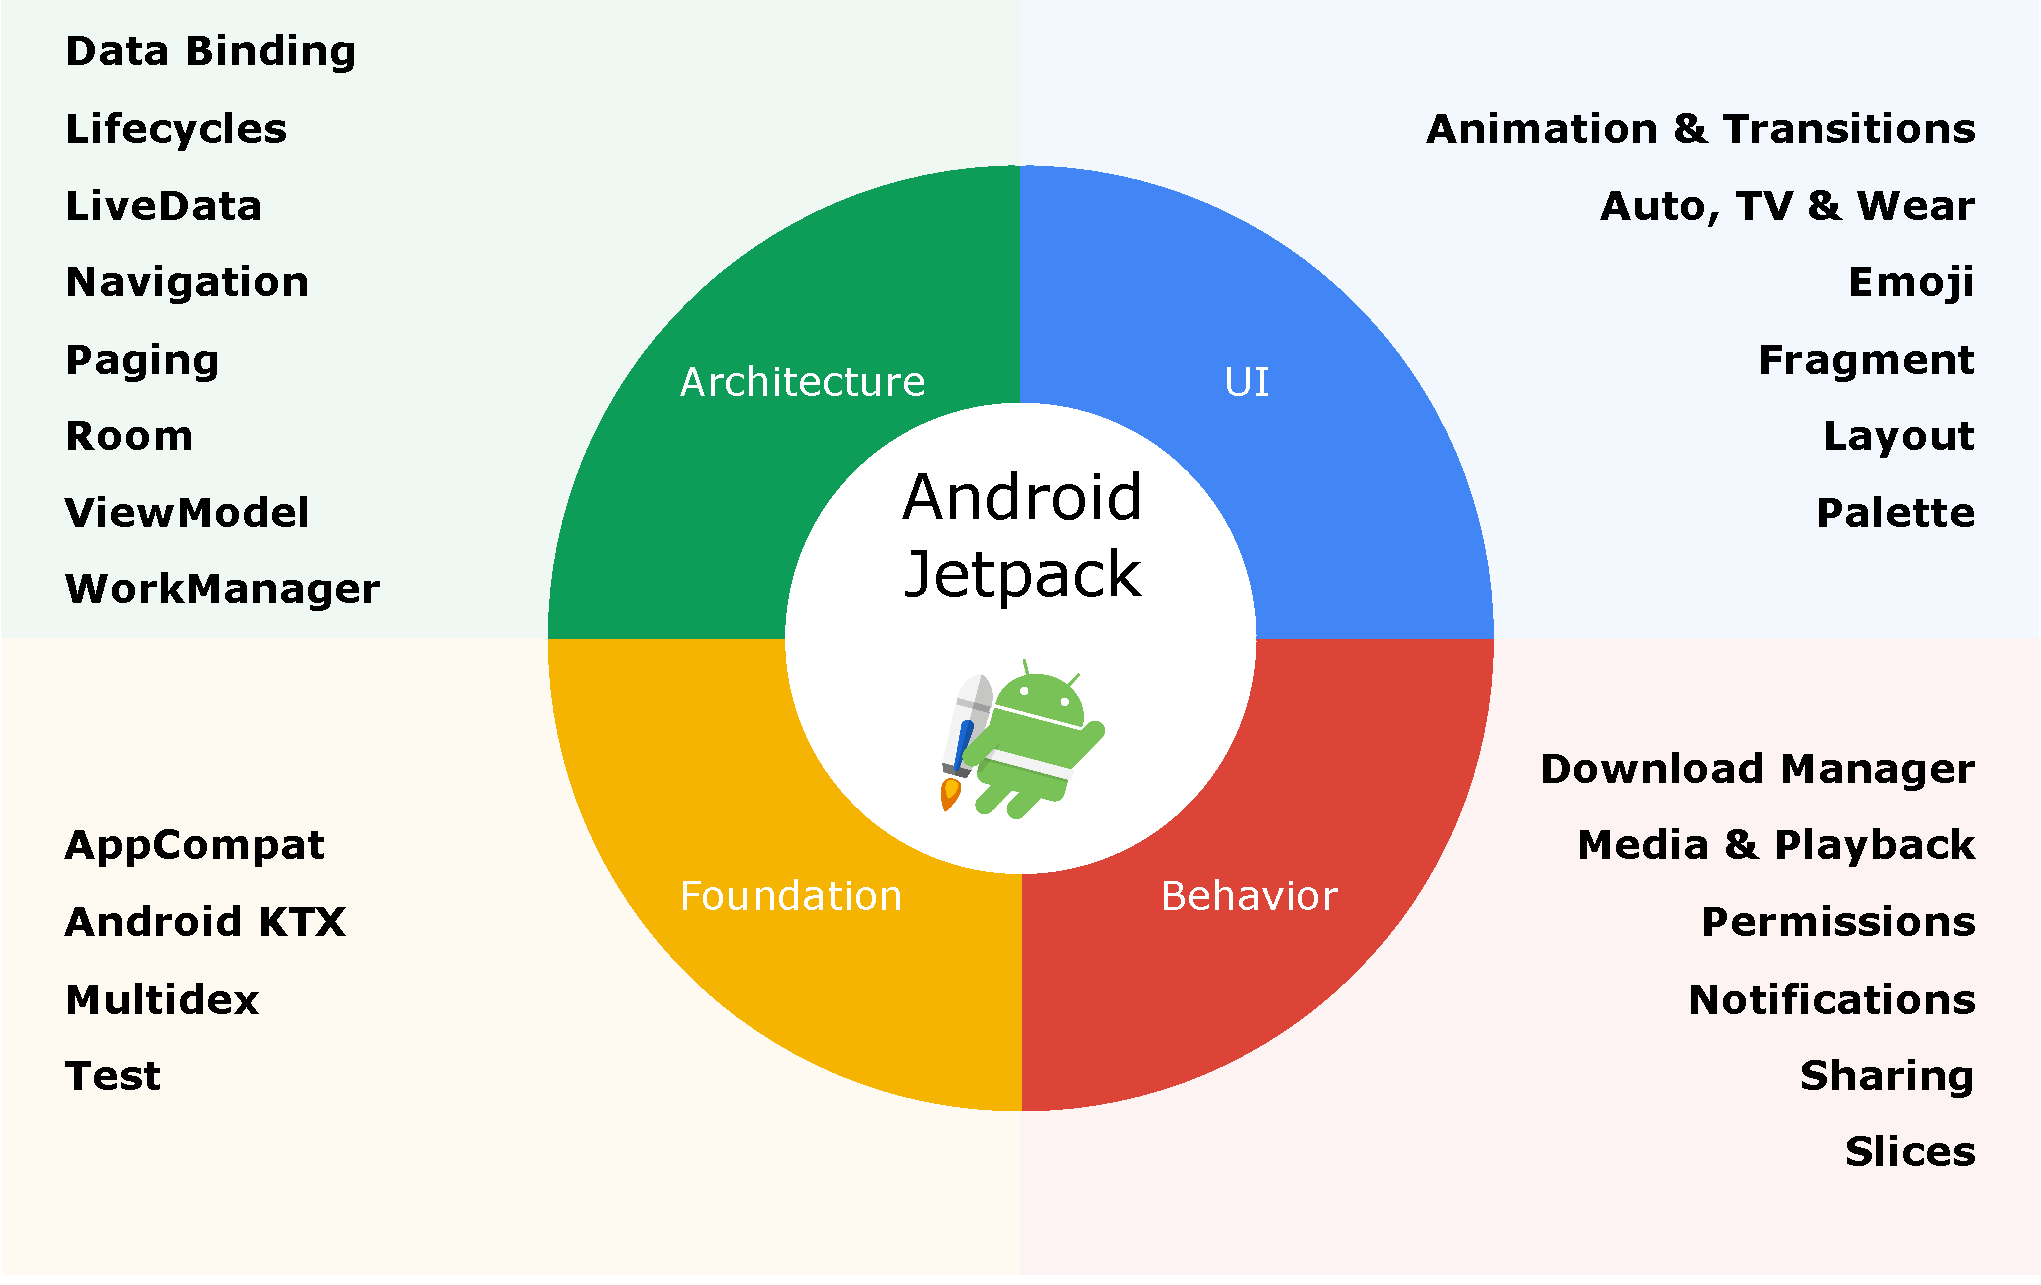
\includegraphics[width=\textwidth]{images/AndroidJetpackUebersicht.drawio.pdf}
	\caption{Überblick über die Komponenten von Android Jetpack \cite{android_jetpack_ueberblick}}
	\label{fig:AndroidJetpackUebersicht}
\end{figure}

Android Jetpack ist eine Sammlung von Bibliotheken und soll Entwicklern*innen dabei helfen, Best Practices zu befolgen, Boilerplate-Code zu reduzieren und Code zu schreiben, der über alle Android-Versionen und -Geräte hinweg konsistent funktioniert \cite{android_jetpack}. Da die Komponenten so aufgebaut sind, dass ihre Funktionalität versionsunabhängig zur Verfügung steht, ist die Abwärtskompatibilität gewährleistet \cite{android_jetpack_ueberblick}. Damit haben Entwickler*innen mehr Zeit sich auf den Code zu konzentrieren, der für ihre App wichtig ist, um leichter und schneller, robuste und hochwertige Apps zu entwickeln. 

Android Jetpack verwaltet also Aktivitäten wie Hintergrundaufgaben, Navigation und Lebenszyklusmanagement. Jetpack ist für eine gute Zusammenarbeit mit Kotlin konzipiert und zusätzlich kann mit der Komponente Android KTX einiges an Code eingespart werden. Die von Jetpack verwalteten Aktivitäten, Kotlin und die Komponenten Android KTX tragen daher gemeinsam dazu bei den Boilerplate-Code zu eliminieren. \cite{android_whats_new}

Die Android Jetpack-Komponenten sind als sogenannte "unbundled" Libraries bereitgestellt und sind nicht Teil der Android-Plattform. Dadurch können Updates der Libraries auch unabhängig und öfter durchgeführt werden \cite{androidx_releases}. Diese Libraries wurden alle in den neuen androidx.* Namespace verschoben und können einzeln oder auch in Kombination verwendet werden. \cite{android_jetpack_ueberblick} Daher ist AndroidX eine wesentliche Verbesserung zu der ursprünglichen Android Support Library, welche nicht mehr gewartet wird \cite{androidx_ueberblick}.


\section{Android Jetpack-Komponenten}

Um mit den Android Jetpack-Komponenten zu starten, ist es wichtig zu wissen, wo diese zu einem Projekt hinzugefügt werden können. Die gesamten Jetpack-Komponenten sind im Google Maven repository\footnote{\url{https://maven.google.com/web/index.html} Zugriff am 10.12.2022} verfügbar. \cite{android_jetpack_getting_started}

Wird in Android Studio ein neues Android Compose Projekt angelegt, so wird die \lstinline{settings.gradle} Datei wie in Listing \ref{lst:settings.gradle} ersichtlich automatisch angelegt.

\begin{lstlisting}[frame=lines, caption=\lstinline{settings.gradle} Datei, captionpos=b, label = lst:settings.gradle, language=Groovy, showstringspaces=false]
pluginManagement {
    repositories {
        gradlePluginPortal()
        google()
        mavenCentral()
    }
}
dependencyResolutionManagement {
    repositoriesMode.set(RepositoriesMode.FAIL_ON_PROJECT_REPOS)
    repositories {
        google()
        mavenCentral()
    }
}
rootProject.name = "TestApp"
include ':app'
\end{lstlisting}

Hier ist es wichtig, dass das \lstinline{google()} repository in dem \lstinline{repositories} Block, welcher sich im \lstinline{dependencyResolutionManagement} Block befindet, eingetragen ist, um Jetpack-Komponenten vom Google Maven repository verwenden zu können. Anschließend ist es möglich in der \lstinline{build.gradle} Datei im \lstinline{app} Ordner, Jetpack-Komponenten hinzuzufügen. \cite{android_jetpack_getting_started} Um zum Beispiel die CameraX Komponente hinzuzufügen, wird innerhalb des Blocks der \lstinline{dependencies} die folgende Codezeile hinzugefügt.

\noindent\oldlstinline[language=Groovy]{implementation 'androidx.camera:camera-camera2:1.3.0-alpha02'} 

\noindent Im Listing \ref{lst:build.gradle} ist die \lstinline{build.gradle} Datei aus dem App Ordner mit den Komponenten ersichtlich, die automatisch nach Anlegen des Projekts enthalten sind. Der \lstinline{android} Konfigurationsblock wurde in diesem Listing aufgrund seiner Größe nicht integriert. 

\begin{lstlisting}[frame=lines, caption=\lstinline{build.gradle} Datei im App Ordner, captionpos=b, label = lst:build.gradle, language=Groovy, showstringspaces=false]
plugins {
    id 'com.android.application'
    id 'org.jetbrains.kotlin.android'
    id 'kotlin-kapt'
}

android {
    ...
}

dependencies {
    implementation 'androidx.core:core-ktx:1.9.0'
    implementation 'androidx.lifecycle:lifecycle-runtime-ktx:2.5.1'
    implementation 'androidx.activity:activity-compose:1.6.1'
    implementation "androidx.compose.ui:ui:$compose_ui_version"
    implementation "androidx.compose.ui:ui-tooling-preview:$compose_ui_version"
    implementation 'androidx.compose.material:material:1.3.0'
    testImplementation 'junit:junit:4.13.2'
    androidTestImplementation 'androidx.test.ext:junit:1.1.3'
    androidTestImplementation 'androidx.test.espresso:espresso-core:3.4.0'
    androidTestImplementation "androidx.compose.ui:ui-test-junit4:$compose_ui_version"
    debugImplementation "androidx.compose.ui:ui-tooling:$compose_ui_version"
    debugImplementation "androidx.compose.ui:ui-test-manifest:$compose_ui_version"
}
\end{lstlisting}

Eine gewisse Anzahl an Jetpack Bibliotheken bieten Android KTX Erweiterungen, welche auf der Java-basierten API aufbauen und Kotlin-spezifische Sprachfunktionen nutzen \cite{android_jetpack_getting_started}. Wie schon erwähnt werden die Jetpack Bibliotheken im \lstinline{androidx} Namespace veröffentlicht. Wenn ein Projekt noch die Android Support Library nutzt, kann diese in den \lstinline{androidx} Namespace migriert werden \cite{migrate_to_androidx}.


\subsection{Versionierung}

Die verschiedenen Bibliotheken besitzen drei Zahlen und bei Vorabversionen zusätzlich einen Suffix der die jeweilige Vorabversionsphase angibt. Die erste Zahl von links beginnenden repräsentiert major, die zweite minor und die dritte das Bugfix-Level. Bei Vorabversionen wird hinter diesen drei Zahlen entweder Alpha, Beta oder Release Candidate hinzugefügt. Wobei Alpha für eine stabile Version steht, die jedoch noch nicht alle Features inkludiert hat. Bei Beta Versionen handelt es sich wieder um stabile Versionen, die auch über eine vollständige API-Oberfläche verfügen, jedoch Fehler enthalten können. Release Candidate ist eine voraussichtlich stabile Version mit einer endgültigen API-Oberfläche. Bibliotheken, die keinen Suffix besitzen sind sogenannte Stable Versionen, die stabil laufen und alle Funktionen implementiert haben. Eine Bibliothek kann auch mehrere Versionen gleichzeitig besitzen, wobei jede Version ein anderes Release-Stadium hat. Eine Bibliothek kann zum Beispiel eine Stabile, eine Alpha und eine Beta Version gleichzeitig besitzen. \cite{androidx_releases}


\subsection{Core}



\subsection{Activity}

In einer Android Anwendung sind Activities eine wesentliche Komponente. Die Art und Weise, wie Activities gestartet und zusammengestellt werden, ist ein grundlegender Teil des Anwendungsmodells der Plattform. Während in anderen Programmierstilen Apps mit einer \lstinline{main()}-Methode gestartet werden, gibt es im Android-System ein anderes Konzept für den Start von Code in der App. Android initiiert den Code in einer \lstinline{Activity}-Instanz, indem es bestimmte Callback-Methoden aufruft, die bestimmten Phasen des Lebenszyklus entsprechen. \cite{android_activities}

Die Interaktion mit einer App beginnt nicht immer an derselben Stelle. Wird zum Beispiel eine E-Mail-App vom Startbildschirm aus geöffnet, wird meistens eine Liste von E-Mails angezeigt. Öffnet jedoch eine andere App die E-Mail-App, sieht man möglicherweise den Bildschirm, um eine neue E-Mail zu verfassen. Um diesen Stil zu unterstützen, wurde die \lstinline{Activity} Klasse entwickelt. Wenn also eine App eine andere App aufruft, so wird eine Aktivität in der Ziel-App aufgerufen und nicht die App als Ganzes. Die Activity dient daher als Einstiegspunkt für diese Interaktion. Die meisten Anwendungen enthalten mehrere Screens und bestehen daher aus mehreren Aktivitäten. Meistens ist der erste Screen beim Starten die Hauptaktivität. Jede Aktivität hat die Möglichkeit eine andere Aktivität zu starten. Zum Beispiel wird aus dem Posteingang einer E-Mail-App ein neuer Screen für das Schreiben einer neuen E-Mail gestartet. Obwohl Aktivitäten zusammenarbeiten, besteht in einer App nur eine minimale Abhängigkeit zwischen ihnen. Um Aktivitäten verwenden zu können, müssen Informationen über sie im Manifest der App registriert werden und auch die Lebenszyklen der Aktivitäten verwaltet werden. \cite{android_activities} Seit 2018 geht der Trend für die Strukturierung der In-App Benutzeroberfläche, durch die Einführung der Android-Jetpack Komponente Navigation, zur Single-Activity-App Architektur \cite{android_jetpack_ueberblick}.


\subsection{Lifecycle}

Wenn ein Benutzer innerhalb, aus und zurück in die App navigiert wechseln die Zustände der Aktivität in ihrem Lebenszyklus. Die \lstinline{Activity} Klasse bietet verschiedene Callbacks die der Aktivität mitteilen das sich der Zustand verändert hat. Mit den Lifecycle-Callback Methoden können Entwickler*innen bestimmen, wie sich die Aktivität verhalten soll, wenn die App verlassen wird und später wieder aufgerufen wird. Das heißt jeder Callback kann bestimmte Aufgaben ausführen, die für einen bestimmten Zustandswechsel passen sind. Eine gute Implementierung der Lifecycle-Callbacks machen die App robuster, leistungsfähiger und verhindern unerwünschtes Verhalten, wie in „The activity lifecycle“ beschrieben. \cite{android_lifecycle}

\begin{itemize} 
  \item Absturz der App, wenn bei der Verwendung der App ein Anruf eintrifft oder während der Verwendung zu einer anderen App gewechselt wird.
  \item Verbrauch wertvoller Systemressourcen, wenn die App nicht aktiv verwendet wird.
  \item Der Verlust des Fortschritts, wenn die App verlassen wird und zu einem späteren Zeitpunkt wieder aufgerufen wird.
  \item Absturz oder Verlust des Fortschritts, wenn zwischen Hoch- und Querformat gewechselt wird.
\end{itemize}

Um die Übergänge zwischen den einzelnen Phasen des Activity Lifecycles zu steuern, stellt die \lstinline{Activity}-Klasse ein Set von sieben Callbacks zur Verfügung. Das System ruft jeden dieser Callbacks auf, sobald eine Aktivität einen neuen Zustand erreicht. \cite{android_lifecycle} Die einzelnen Callbacks mit ihren grundlegenden Funktionen sind hier wie im Abschnitt "Activity Lifecycle" aufgeführt \cite{android_activity}.

\begin{itemize} 
  \item \textbf{\lstinline{onCreate()}} \\ 
        Wird aufgerufen, wenn die Aktivität zum ersten Mal erstellt wird. \\
        Es folgt immer \lstinline{onStart()}.
  \item \textbf{\lstinline{onRestart()}} \\ 
        Diese Callback Methode wird aufgerufen, nachdem die Aktivität gestoppt wurde und bevor sie wieder gestartet wird. \\
        Es folgt immer \lstinline{onStart()}.
  \item \textbf{\lstinline{onStart()}} \\ 
        Der Aufruf erfolgt, wenn die Aktivität für den*die Benutzer*in sichtbar wird. \\
        Es folgt immer \lstinline{onResume()}.
  \item \textbf{\lstinline{onResume()}} \\ 
        Wird aufgerufen, wenn die Aktivität beginnt, mit dem*der Benutzer*in zu interagieren und Eingaben gehen direkt an die Aktivität. \\
        Es folgt immer \lstinline{onPause()}.
  \item \textbf{\lstinline{onPause()}} \\ 
        Der Aufruf von \lstinline{onPause()} erfolgt, wenn die Aktivität den Vordergrundstatus verliert, nicht mehr fokussierbar ist oder vor dem Übergang in den Zustand \lstinline{onStop()} oder \lstinline{onDestroy()}. \\
        Wenn die Aktivität wieder in den Vordergrund tritt, folgt \lstinline{onResume()} oder \lstinline{onStop()}, wenn sie für den*die Benutzer*in nicht mehr sichtbar ist. 
  \item \textbf{\lstinline{onStop()}} \\ 
        Dieser Callback wird aufgerufen, wenn die Aktivität für den Benutzer nicht mehr sichtbar ist. Das passiert, wenn eine neue Aktivität gestartet wird, beziehungsweise eine andere Aktivität vor dieses geschoben wird oder diese Aktivität zerstört wird. \\
        Es folgt entweder \lstinline{onRestart()}, wenn die Aktivität zurückkehrt, um damit wieder zu interagieren oder \lstinline{onDestroy()}, wenn die Aktivität verschwindet. 
  \item \textbf{\lstinline{onDestroy()}} \\ 
        Ist der letzte Callback, bevor die Aktivität zerstört wird, entweder weil die Aktivität durch \lstinline{finish()} beendet wird oder weil das System diese Instanz der Aktivität vorübergehend zerstört, um Platz zu sparen.\\
        Nach diesem Callback gibt es logischerweise keine Nachfolger.
\end{itemize}

Abbildung \ref{fig:Aktivitätslebenszyklus} zeigt die verschiedenen Callbacks in einem vereinfachten Aktivitätslebenszyklus. 

\begin{figure}[H]
	\centering
		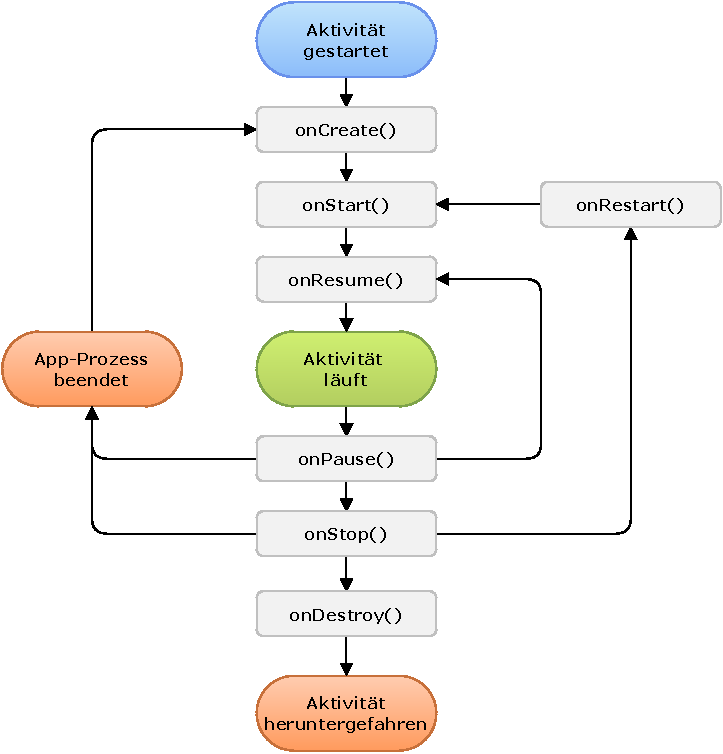
\includegraphics[]{images/Aktivitaetslebenszyklus.drawio.pdf}
	\caption{Callbacks im Aktivitätslebenszyklus \cite{android_lifecycle}}
	\label{fig:Aktivitätslebenszyklus}
\end{figure}

Das \lstinline{androidx.lifecycle}-Paket bietet Klassen und Schnittstellen an, mit denen Komponenten erstellt werden können, die den Lebenszyklus einer Aktivität oder eines Fragments berücksichtigen und ihr Verhalten automatisch an diesen Lebenszyklus anpassen. Diese sogenannten „Lifecycle-Aware Components“ führen, auf Grund einer Änderung des Lebenszyklus einer anderen Aktivität, Aktionen aus. \cite{android_architecture_lifecycle}

Die \lstinline{Lifecycle} Klasse enthält Informationen über den Zustand des Lebenszyklus einer Komponente und ermöglicht anderen Objekten diesen Zustand zu beobachten. Um den Lebenszyklus für eine zugehörige Komponente zu verfolgen, verwendet die \lstinline{Lifecycle} Klasse verschiedene Ereignisse und Zustände. Einerseits die Ereignisse oder Events, die vom Framework und der \lstinline{Lifecycle} Klasse ausgeführt werden und den Callback Ereignissen in den Aktivitäten entsprechen. Andererseits der aktuelle Zustand oder State, der vom \lstinline{Lifecycle} Objekt verfolgt wird. \cite{android_architecture_lifecycle}

\lstinline{LifecycleOwner} ist eine Schnittstelle, die eine Methode hat und gibt an, dass eine Klasse einen Lebenszyklus hat. Die Methode \lstinline{getLifecycle()} muss von der Klasse implementiert werden. Jede Benutzerdefinierte Klasse kann die \lstinline{LifecycleOwner} Schnittstelle implementieren. Fragmente und Aktivitäten im \lstinline{androidx} Namespace implementieren bereits die \lstinline{LifecycleOwner} Schnittstelle. Komponenten die \lstinline{DefaultLifecycleObserver} implementiert haben, arbeiten mit Komponenten die \lstinline{LifecycleOwner} implementiert haben zusammen, weil ein Owner seinen Lebenszyklus zur Beobachtung freigibt und sich ein Observer zur Beobachtung anmelden kann. \cite{android_architecture_lifecycle} Der \lstinline{DefaultLifecycleObserver} ist also eine sogenannte Callback-Schnittstelle zum Abhören von \lstinline{LifecycleOwner} Zustandsänderungen \cite{DefaultLifecycleObserver}.

Im Listing \ref{lst:LifecycleObserverUndLifecycleOwner} ist die Klasse \lstinline{MyObserver}, die das Interface \lstinline{DefaultLifecycleObserver} implementiert, um den Lebenszyklusstatus des \lstinline{LifecycleOwners} zu überwachen und die beiden Methoden \lstinline{onResume} und \lstinline{onPause} überschreibt, zu sehen. Zusätzlich wird über das Objekt \lstinline{myLifecycleOwner}, welches die Schnittstelle \lstinline{LifecycleOwners} implementiert, ein Observer hinzugefügt, indem die Methode \lstinline{addObserver()} der \lstinline{Lifecycle}-Klasse aufgerufen wird und eine Instanz des Observers übergeben wird \cite{android_architecture_lifecycle}.

\begin{lstlisting}[frame=lines, caption=Beispeilcode für \lstinline{LifecycleObserver} und \lstinline{LifecycleOwner} \cite{android_architecture_lifecycle}, captionpos=b, label = lst:LifecycleObserverUndLifecycleOwner, language=Kotlin, showstringspaces=false]
class MyObserver : DefaultLifecycleObserver {
    override fun onResume(owner: LifecycleOwner) {
        connect()
    }

    override fun onPause(owner: LifecycleOwner) {
        disconnect()
    }
}

myLifecycleOwner.getLifecycle().addObserver(MyObserver())
\end{lstlisting}

Einige Anwendungsfälle für die Verwendung von „lifecycle-aware components“, wie in „Use cases for lifecycle-aware components“ beschrieben sind zum Beispiel: \cite{android_architecture_lifecycle}
\begin{itemize}
  \item Umschalten zwischen grob- und feinkörnigen Standortaktualisierungen.
  \item Anhalten und Starten der Videopufferung.
  \item Starten und Stoppen der Netzwerkverbindung.
  \item Anhalten und Fortsetzen von animierten Zeichenflächen.
\end{itemize}

\subsubsection{Viewmodel}

Die Klasse \lstinline{ViewModel} hält den Status für die Geschäftslogik oder die Bildschirmebene. Sie stellt den Zustand der Benutzeroberfläche zur Verfügung und kapselt die Geschäftslogik \cite{viewmodel_overview}. Ein \lstinline{ViewModel} ist für die Vorbereitung und Verwaltung der Daten für eine Activity oder ein Fragment verantwortlich und übernimmt auch die Kommunikation zwischen Activity und Fragment mit dem Rest der Anwendung \cite{viewmodel}. Der Hauptvorteil der Arbeitsweise von \lstinline{ViewModel} ist, dass der Status zwischengespeichert wird und auch bei Konfigurationsänderungen beibehalten wird. Die Benutzeroberfläche muss daher die Daten nicht erneut abrufen, wenn zwischen Aktivitäten navigiert wird. Dabei handelt es sich zum Beispiel um das Drehen des Bildschirms. \cite{viewmodel_overview}

Eine Alternative dazu wäre eine einfache Klasse, die alle Daten der Benutzeroberfläche enthält. Wenn jedoch wird er zwischen den Aktivitäten navigiert wird, kann es zu einem Datenverlust kommen. Um dieses Problem zu beheben bietet \lstinline{ViewModel} ein API, welche auch für Datenpersistenz sorgt. \cite{viewmodel_overview}

Einem \lstinline{ViewModel}, das instanziiert wird, wird ein Objekt übergeben, dass die Schnittstelle \lstinline{ViewModelStoreOwner} implementiert. Das \lstinline{ViewModel} wird anschließend in den Lebenszyklus des \lstinline{ViewModelStoreOwner} integriert und bleibt so lange im Speicher, bis sein \lstinline{ViewModelStoreOwner} dauerhaft verschwindet. Dies kann in den folgenden Fällen auftreten, wie in „The lifecycle of a ViewModel“ erwähnt. \cite{viewmodel_overview}

\begin{itemize}
  \item Im Falle einer Aktivität, wenn sie beendet ist.
  \item Im Falle eines Fragments, wenn es sich loslöst.
  \item Im Falle eines Navigationseintrags, wenn er aus dem Backstack entfernt wird.
\end{itemize}

Abbildung \ref{fig:ViewModelLebenszyklus} zeigt sowohl die unterschiedlichen Zustände vom Lebenszyklus einer Aktivität als auch die Lebensdauer des \lstinline{ViewModels}, während die Aktivität eine Rotation durchläuft und dann beendet wird. Dabei existiert das \lstinline{ViewModel} von der ersten Anforderung bis zur Beendigung und Zerstörung der Aktivität. \cite{viewmodel_overview}

\begin{figure}[H]
	\centering
		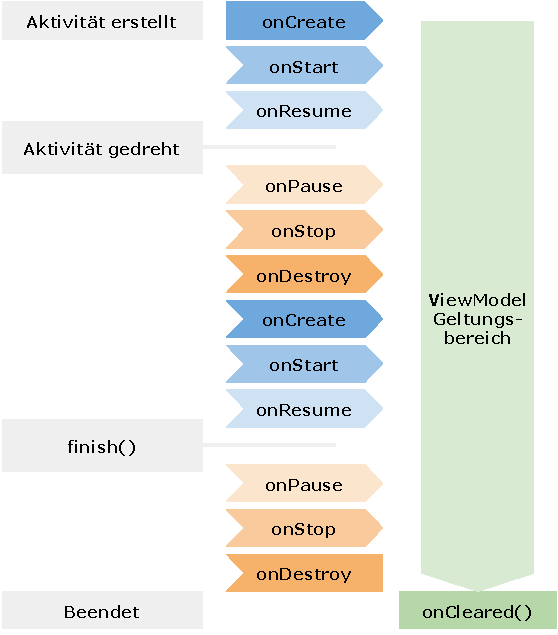
\includegraphics[]{images/ViewModelLifecycle.drawio.pdf}
	\caption{Lebenszyklus eines \lstinline{ViewModels} \cite{viewmodel_overview}}
	\label{fig:ViewModelLebenszyklus}
\end{figure}

Die Schnittstelle \lstinline{ViewModelStoreOwner} besitzt eine Reihe von direkten oder indirekten Unterklassen. ComponentActivity, Fragment, und NavBackStackEntry sind direkte Unterklassen. \cite{viewmodel_overview}

Die asynchrone Arbeit im \lstinline{ViewModel} wird auch fortgesetzt, wenn ein Fragment oder eine Aktivität auf die das \lstinline{ViewModel} skaliert ist, zerstört werden \cite{viewmodel_overview}.

Da die UI-Schicht in bestimmten Fällen auch Geschäftslogik enthalten kann, ist das \lstinline{ViewModel} geeignet diese zu behandeln. Muss Geschäftslogik zur Änderung von Daten angewendet werden, ist das \lstinline{ViewModel} auch für diese Bearbeitung von Ereignissen zuständig. \cite{viewmodel_overview}

\subsubsection{LiveData}

Die Informationen, die das ViewModel für eine Aktivität oder ein Fragment speichert, können vom ViewModel über LiveData zur Verfügung gestellt werden. \lstinline{LiveData} ist eine Klasse, die beobachtbar ist und Daten hält. LiveData ist dabei lebenszyklusorientiert und berücksichtigt den Lebenszyklus von Aktivitäten und Fragmenten nur dann, wenn sich diese auch in einem aktiven Lebenszyklus-Zustand befinden. \cite{livedata_overview}

LiveData nimmt zu einem Obserever, der durch die Klasse \lstinline{Observer} repräsentiert wrid, nur Verbindung auf, wenn dieser in einem aktiven Zustand ist, also sein Lebenszyklus sich im Zustand \lstinline{STARTED} or \lstinline{RESUMED} befindet. Inaktive Observer werden nicht über Updates informiert. \cite{livedata_overview}

Ein Observer kann mit einem Objekt registriert werden, das die Schnittstelle \lstinline{LifecycleOwner} implementiert. Dadurch wird der Observer auch wieder sofort entfernt, wenn das entsprechende \lstinline{Lifecycle}-Objekt in den Status \lstinline{DESTROYED} wechselt. Für Aktivitäten und Fragmente ist das besonders nützlich, weil \lstinline{LiveData}-Objekte sicher beobachtet werden und keine Lecks entstehen. Die Verwendung von LiveData hat folgende Vorteile, wie im Abschnitt „The advantages of using LiveData“ aufgeführt. \cite{livedata_overview}

\begin{itemize} 
  \item \textbf{Sicherstellung, der Übereinstimmung von Benutzeroberfläche und Datenzustand} \\ 
        Die Benutzeroberfläche muss nicht jedes Mal aktualisiert werden, wenn sich Anwendungsdaten ändern, denn diesen Vorgang übernimmt der Observer. 
  \item \textbf{Keine Speicherlecks} \\ 
        Observer sind an \lstinline{Lifecycle}-Objekte gebunden und geben ihre Ressourcen frei, wenn ihr zugehöriger Lifecycle zerstört wird.
  \item \textbf{Keine Abstürze aufgrund von gestoppten Aktivitäten} \\ 
        Wenn der Lebenszyklus des Observers inaktiv ist, beispielsweise wenn sich die Aktivität im Backstack befindet, dann erhält er keine LiveData-Ereignisse.
  \item \textbf{Keine manuelle Verwaltung des Lebenszyklus mehr} \\ 
        UI-Komponenten beobachten nur relevanten Daten und die Beobachtung wird weder stoppen noch fortgesetzt. LiveData verwaltet alles automatisch, da die relevanten Änderungen des Lebenszyklusstatus während der Beobachtung bekannt sind.
  \item \textbf{Immer aktuelle Daten} \\ 
        Ein Lebenszyklus der inaktiv wird, erhält die neuesten Daten, sobald er wieder aktiv wird.
  \item \textbf{Ordnungsgemäße Konfigurationsänderungen} \\ 
        Wird eine Aktivität oder ein Fragment aufgrund einer Konfigurationsänderung, wie zum Beispiel der Bildschirmdrehung, neu erstellt, erhält es sofort die aktuellsten verfügbaren Daten.
  \item \textbf{Gemeinsame Nutzung von Ressourcen} \\ 
        Mit dem Singleton Pattern kann ein \lstinline{LiveData}-Objekt erweitert werden, um Systemdienste so zu verpacken, dass sie in der Anwendung gemeinsam genutzt werden können. Das \lstinline{LiveData}-Objekt verbindet sich einmal mit dem Systemdienst und jeder Beobachter, der die Ressource benötigt, kann das Objekt beobachten. 
\end{itemize}


\subsection{Paging}

Beim Arbeiten mit größeren Datensätzen, die aus dem lokalen Speicher oder über das Netzwerk geladen und anschließend angezeigt werden, ist der Einsatz der Paging-Bibliothek hilfreich. Paging ermöglicht es Netzwerkbandbreite, aber auch Systemressourcen effizienter zu nutzen. Die Komponenten der Paging-Bibliothek lassen sich problemlos mit anderen Jetpack-Komponenten kombinieren und bieten Kotlin-Support. \cite{paging_overview}

Die Paging-Bibliothek enthält die folgenden Funktionen, wie in „Benefits of using the Paging library“ beschrieben \cite{paging_overview}.

\begin{itemize} 
  \item Durch In-Memory-Caching wird sichergestellt, dass die Anwendung bei der Arbeit mit ausgelagerten Daten die Systemressourcen effizient nutzt.
  \item Effiziente Nutzung der Netzwerkbandbreite und Systemressourcen durch integrierte Anforderungs-Deduplizierung.
  \item Konfigurierbare \lstinline{RecyclerView}-Adapter die, wenn der Benutzer zum Ende der geladenen Daten scrollt, automatisch Daten anfordern.
  \item Untersützt Kotlin Coroutines und Flow sowie LiveData und RxJava.
  \item Integrierte Unterstützung für die Fehlerbehandlung, inklusive Aktualisierungs- und Wiederholungsfunktionen.
\end{itemize}

Die Paging-Bibliothek ist in die Android-App-Architektur direkt integrierbar, wobei die Komponenten der Bibliothek in einer App in drei Schichten arbeiten. Bei den drei Schichten handelt es sich um die Repository-Schicht, die ViewModel-Schicht und die UI-Schicht, wie auch in Abbildung \ref{fig:PagingBibliothekArchitektur} ersichtlich ist. \cite{paging_overview} 

\begin{figure}[H]
	\centering
		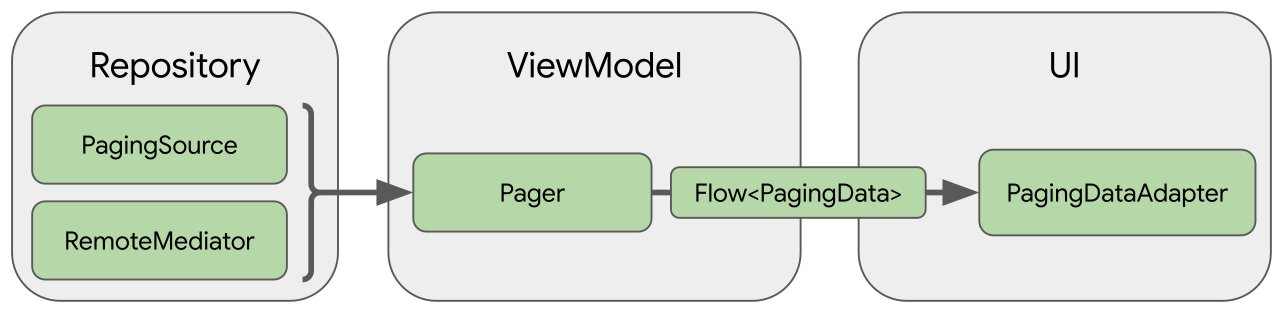
\includegraphics[width=\textwidth]{images/PagingBibliothekArchitektur.jpg}
	\caption{Architektur der Paging-Bibliothek \cite{paging_overview}}
	\label{fig:PagingBibliothekArchitektur}
\end{figure}

\noindent\textbf{Repository-Schicht} \\
Die wichtigste Komponente in der Repository-Schicht ist \lstinline{PagingSource}. Ein \lstinline{PagingSource}-Objekt legt eine Datenquelle fest und definiert, wie die Daten aus dieser Quelle abgerufen werden. \cite{paging_overview}

Eine weitere Komponente ist der \lstinline{RemoteMediator}, welcher das Paging aus einer mehrschichtigen Datenquelle, zum Beispiel eine Netzwerkdatenquelle mit einem lokalen Datenbank-Cache, verwaltet \cite{paging_overview}. 

\noindent\textbf{ViewModel-Schicht} \\
Die \lstinline{Pager}-Komponente bietet eine öffentliche API zur Erstellung von Instanzen von \lstinline{PagingData}, die in reaktiven Streams auf der Grundlage eines \lstinline{PagingSource}-Objekts und eines \lstinline{PagingConfig}-Konfigurationsobjekts dargestellt werden \cite{paging_overview}.

\lstinline{PagingData} ist eine Komponente, welche die \lstinline{ViewModel}-Schicht mit der Benutzeroberfläche verbindet. Ein \lstinline{PagingData}-Objekt fragt ein \lstinline{PagingSource}-Objekt ab und speichert das Ergebnis \cite{paging_overview}. 

\noindent\textbf{UI-Schicht} \\
Der \lstinline{PagingDataAdapter} in der UI-Schicht ist ein RecyclerView-Adapter, der die Paging Daten verarbeitet. Bei Verwendung von Jetpack Compose für das UI wird \lstinline{collectAsLazyPagingItems()} verwendet, um die Daten entweder in einer Lazy list oder in einem Lazy grid anzuzeigen. \cite{paging_overview}

\subsection{DataStore}

Bei der DataStore-Bibliothek handelt es sich um eine neue und verbesserte Datenspeicherlösung, welche die SharedPreferences ersetzen soll. Dabei werden die Daten unter Verwendung von Kotlin Coroutines und Flow asynchron, konsistent und transaktional gespeichert und dadurch die meisten Nachteile von SharedPreferences beseitigt. \cite{datastore_releases} 

Mit der DataStore-Bibliothek sind zwei verschiedene Implementierungen möglich. Bei \mbox{\textbf{Preferences DataStore}} werden Daten mithilfe von Schlüsseln gespeichert und auf sie zugegriffen, wobei kein vordefiniertes Schema verwendet werden muss und es keine Typensicherheit bietet. Bei \mbox{\textbf{Proto DataStore}} werden die Daten als Instanzen eines benutzerdefinierten Datentyps gespeichert. Diese Art der Implementierung benötigt die Definition eines Schemas unter Verwendung von Protokollpuffern, dafür wird aber Typsicherheit geboten. \cite{datastore}

DataStore eignet sich gut für kleine, einfache Datensätze und es ist darauf zu achten, dass es keine partiellen Aktualisierungen oder referenzielle Integrität unterstützt. Wenn mit großen oder komplexen Datensätzen gearbeitet wird oder partielle Aktualisierungen oder referenzielle Integrität benötigt wird, dann sollte Room anstelle von DataStore verwendet werden. \cite{datastore}


\subsection{Work}

Zuverlässige und akkuschonende Verarbeitung im Hintergrund sind eine große Herausforderung. Zusätzlich boten die verschiedenen Android-Versionen unterschiedliche Tools für Arbeiten im Hintergrund. Die Netzwerk- oder Speicherverfügbarkeit abzuhören und das automatische Wiederholen von Aufgaben war zum Beispiel mit viel Arbeit verbunden. \cite{workmanager_stable_release}

WorkManager erleichtert die Arbeit im Hintergrund und berücksichtigt Einschränkungen, wie Akku-Optimierung, Speicherplatz oder Netzwerkverfügbarkeit. Der WorkManager führt diese Aufgaben nur aus, sofern die jeweiligen Bedingungen erfüllt sind. \cite{workmanager_stable_release} Die WorkManager-API stellt eine verbesserte Alternative für die Verwaltung von Hintergrundaufgaben in Android dar und löst damit alle früheren APIs in diesem Bereich ab, wie beispielsweise FirebaseJobDispatcher, GcmNetworkManager und Job Scheduler \cite{workmanager}. 

Die meisten Hintergrundverarbeitungen werden am besten durch persistente Arbeit erreicht, die auch nach einem Neustart der Anwendung oder des Systems geplant bleibt. WorkManager wird als Lösung für Hintergrundverarbeitung und daher auch für persistente Arbeit empfohlen. \cite{workmanager}

WorkManager kann folgende drei Arten von persistenter Arbeit verwalten, wie in „Types of persistent work“ aufgeführt. \cite{workmanager}

\begin{itemize} 
  \item \textbf{Immediate} \\ 
        Sind Aufgaben, die sofort beginnen und zeitnah abgeschlossen werden müssen und auch beschleunigt werden können. Diese Aufgaben laufen einmalig. 
  \item \textbf{Long Running} \\ 
        Hierbei handelt es sich um Aufgaben, die länger dauern können, möglicherweise länger als 10 Minuten und einmalig oder periodisch ablaufen können. 
  \item \textbf{Deferrable} \\ 
        Sind geplante Aufgaben, die zu einem späteren Zeitpunkt beginnen und einmalig oder periodisch ausgeführt werden können. 
\end{itemize}

Neben der einfacheren und einheitlicheren API bietet der WorkManager auch eine Reihe andere wichtiger Vorteile \cite{workmanager}. 

\noindent\textbf{Arbeitsbeschränkungen} \\
Mithilfe von Arbeitseinschränkungen ist es möglich die Bedingungen für die Ausführung der Arbeit zu definieren. Zum Beispiel soll die Arbeit nur ausgeführt werden, wenn sich das Gerät in einem Netzwerk befindet, das nicht gebührenpflichtig ist, wenn sich das Gerät im Leerlauf befindet oder wenn der Akku ausreichend geladen ist. \cite{workmanager}

\noindent\textbf{Robuste Planung} \\
Einmalige oder wiederkehrende Arbeiten können mit WorkManager flexible geplant, gekennzeichnet und benannt werden, sodass austauschbare Arbeiten entstehen. Diese Arbeiten werden in einer internen verwalteten SQLite-Datenbank gespeichert und bleiben durch den WorkManager auch nach einem Neustart des Geräts erhalten. Zusätzlich hält sich der WorkManager an Energiesparfunktionen und bewährte Verfahren wie den Doze-Modus. \cite{workmanager}

\noindent\textbf{Beschleunigte Arbeit} \\
Sofortige Arbeiten können mit WorkManager zur Ausführung im Hintergrund geplant werden. Beschleunigte Arbeit wird innerhalb weniger Minuten abgeschlossen und sollte für Aufgaben verwendet werden, die für den Benutzer wichtig sind. \cite{workmanager}

\noindent\textbf{Flexible Wiederholungsregelungen} \\
Wenn die Arbeit fehlschlägt, bietet WorkManager flexible Wiederholungsrichtlinien inklusive einer konfigurierbaren exponentiellen Backoff-Richtline \cite{workmanager}. 

\noindent\textbf{Arbeitsverkettung} \\
Bei komplexen, zusammenhängenden Arbeiten können einzelne Arbeitsaufgaben verkettet werden und es kann gesteuert werden welche Teile nacheinander und welche parallel ablaufen sollen. Ausgabedaten werden bei der Verkettung automatisch von einer Arbeitsaufgabe an die nächste übergeben. \cite{workmanager}

\noindent\textbf{Integrierte Threading-Interoperabilität} \\
WorkManager kann problemlos in Coroutines und RxJava integriert werden und bietet die Möglichkeit, eigene asynchrone APIs einzubinden \cite{workmanager}.


\subsection{Room}

Bei Room handelt es sich um eine Database Object Mapping Bibliothek, die den Datenbankzugriff in Android Anwendungen erleichtert. Room stellt APIs zur Abfrage der Datenbank und zur Überprüfung dieser Abfragen während der Kompilierungszeit zur Verfügung. \cite{androidx.room} Room stellt eine Schicht zwischen Anwendung und SQLite bereit, die es ermöglicht, auf die Datenbank zu zugreifen, ohne sich um die Details der SQLite-Implementation kümmern zu müssen, während dennoch die volle Leistung von SQLite und die Typsicherheit von Java und Kotlin SQL Query Buildern genutzt werden kann \cite{androidx.room}, \cite{room}. Außerdem hat Room Annotations, die wiederholenden und fehleranfälligen Boilerplate-Code minimieren und optimierte Migrationspfade für Datenbanken. Aufgrund der Vorteile, die diese Bibliothek bietet, wird empfohlen Room zu verwenden, anstatt die SQLite-APIs direkt zu nutzen. \cite{room}

Die drei wichtigsten Komponenten von Room sind die Room Datenbank, Data Access Objects (DAOs) und Entities, deren Beziehungen untereinander in Abbildung \ref{fig:RoomArchitektur} zu sehen sind. Die Datenbank stellt der Anwendung Instanzen der DAOs zu Verfügung, welche mit der Datenbank verknüpft sind. Die App kann diese DAOs verwenden, um Daten aus der Datenbank als Instanzen der zugehörigen Daten-Entitätsobjekte abzurufen. Außerdem kann die Anwendung die definierten Daten-Entities verwenden, um Zeilen aus den entsprechenden Tabellen zu aktualisieren, einzufügen oder zu löschen. 

\begin{figure}[H]
	\centering
		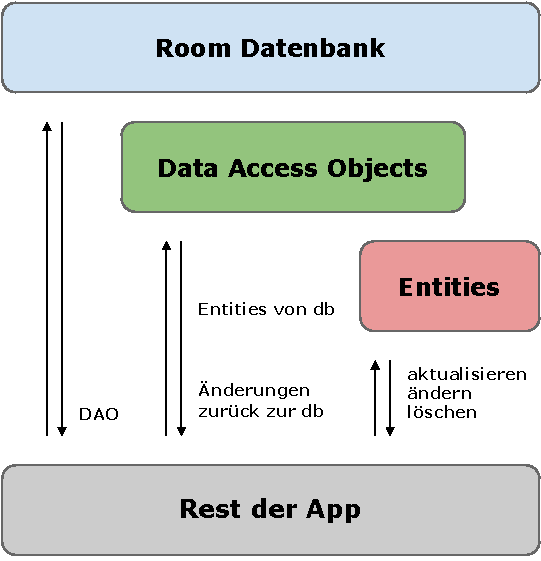
\includegraphics[]{images/RoomArchitektur.drawio.pdf}
	\caption{Architektur der Room-Bibliothek \cite{room}}
	\label{fig:RoomArchitektur}
\end{figure}

\noindent\textbf{Data entity} \\
Entitäten werden definiert, um Objekte darzustellen, die gespeichert werden sollen. Dabei entspricht jede Entität einer Tabelle in der Datenbank und jede Instanz stellt eine Datenzeile dar. Der Vorteil bei der Verwendung von Room-Entitäten ist, dass ein Datenbankschema definierbar ist, ohne SQL-Code schreiben zu müssen. \cite{room_entities} 

Jede Room-Entität ist eine Klasse, die mit \lstinline{@Entity} annotiert ist und enthält Felder für jede Spalte in der entsprechenden Tabelle. Eine Room-Entität muss einen Primärschlüssel haben. Eine oder mehre Spalten können dabei mit \lstinline{@PrimaryKey} gekennzeichnet werden, welche dann den Primärschlüssel bilden. Das Listing \ref{lst:EntityCode} zeigt eine einfache Room-Entität, die eine Tabelle User mit den Spalten ID, Vorname und Nachname definiert, wobei die Spalte ID der Primärschlüssel ist. \cite{room_entities}

\begin{lstlisting}[frame=lines, caption=Code einer Room Entität \cite{room_entities}, captionpos=b, label = lst:EntityCode, language=Kotlin, showstringspaces=false]
@Entity
data class User(
    @PrimaryKey val id: Int,
    val firstName: String?,
    val lastName: String?
)
\end{lstlisting}

\noindent\textbf{DAO} \\
Zum Speichern der Daten in der Anwendung, werden DAOs definiert, wobei jedes DAO Methoden enthält, die einen abstrakten Zugriff auf die Datenbank der App ermöglichen. DAOs erleichtern das Simulieren von Datenbankzugriffen beim Testen der App. \cite{room_daos}

Ein DAO kann als Schnittstelle oder abstrakte Klasse definiert werden, wobei normalerweise Schnittstellen verwendet werden. DAOs werden immer mit \lstinline{@Dao} annotiert. Um Datenbankinteraktionen zu definieren, gibt es zwei verschiedene Arten von DAO-Methoden. Einerseits die Convenience-Methoden, welche das Einfügen, Aktualisieren und Löschen von Zeilen in der Datenbank ermöglichen ohne SQL-Code zu schreiben. Andererseits die Query-Methoden, mit denen durch eigene SQL-Anweisungen Daten aus der Datenbank abgefragt werden können oder komplexere Einfügungen, Aktualisierungen und Löschungen durchgeführt werden können und sie dabei als DAO-Methoden darzustellen. Das Listing \ref{lst:DaoCode} zeigt ein einfaches DAO als \lstinline{UserDao} Schnittstelle, welche sowohl die Convenience-Methoden \lstinline{@Insert} und \lstinline{@Delete}, als auch eine Query-Methode, die mittels eigenem SQL-Code alle User aus der Datenbank abruft, beinhaltet. \cite{room_daos}

\begin{lstlisting}[frame=lines, caption=Code eines DAOs \cite{room_daos}, captionpos=b, label = lst:DaoCode, language=Kotlin, showstringspaces=false]
@Dao
interface UserDao {
    @Insert
    fun insertAll(vararg users: User)

    @Delete
    fun delete(user: User)

    @Query("SELECT * FROM user")
    fun getAll(): List<User>
}
\end{lstlisting}

\noindent\textbf{Datenbank} \\
Die Datenbankklasse enthält die Datenbank, welche als Hauptzugriffspunkt für die Verbindung zu den persistierten Daten in der App dient. Diese Klasse muss eine abstrakte Klasse sein, die \lstinline{RoomDatabase} erweitert und eine \lstinline{@Database}-Annotation haben, welche ein Entity-Array enthält, das alle Data entities auflistet, die mit der Datenbank verbunden sind. Die Datenbankklasse muss für jede DAO-Klasse, die mit der Datenbank verbunden ist, eine abstrakte Methode definieren, die keine Argumente hat und eine Instanz der DAO-Klasse zurückgibt. Im Listing \ref{lst:DatenbankCode} ist die abstrakte Klasse \lstinline{AppDatabase}, welche die \lstinline{RoomDatabase}-Klasse erweitert, mit \lstinline{@Database} annotiert ist und eine abstrakte Methode für das \lstinline{UserDao} definiert, zu sehen. \cite{room}

\begin{lstlisting}[frame=lines, caption=Code der Room Datenbank \cite{room}, captionpos=b, label = lst:DatenbankCode, language=Kotlin, showstringspaces=false]
@Database(entities = [User::class], version = 1)
abstract class AppDatabase : RoomDatabase() {
    abstract fun userDao(): UserDao
}
\end{lstlisting}



\subsection{Compose}
\subsection{Navigation}



\chapter{Schluss}
\section{Zusammenfassung}
Wichtigsten Aussagen der Arbeit wiederholen und miteinander in Beziehung bringen

\section{Bewertung und Ausblick}
Bewertung der verschiedenen Faktoren und Erkenntnisse \\
Ideen für weitere Arbeiten

\newpage

% --- Bibliography ------------------------------------------------------

%IEEE Citation [1]:
\bibliographystyle{IEEEtran}
%for alphanumeric citation eg.: [ABC19]
%\bibliographystyle{alpha}

% List references I definitely want in the bibliography,
% regardless of whether or not I cite them in the thesis.

\newpage
\addcontentsline{toc}{chapter}{Bibliographie}
\bibliography{thesis}

\newpage

% --- List of Figures ----------------------------------------------------

\addcontentsline{toc}{chapter}{Abbildungen}
\listoffigures


% --- List of Tables -----------------------------------------------------

\newpage
\addcontentsline{toc}{chapter}{Tabellen}
\listoftables

% --- Appendix A -----------------------------------------------------

\newpage
\backmatter
\appendix
\begin{appendices}
\chapter{Appendix}

(Hier können Schaltpläne, Programme usw. eingefügt werden.)

\clearpage
\end{appendices}

\end{document}
